\section{Syntax Analysis}
The second part of the compiler parses the lexical tokens outputted by the lexer. 
This part of the compiler is called the parser. 
The parser works by taking a sequence of lexical tokens, and generating a parse tree or transforming them into an abstract syntax tree. 

\subsection{Output data types}
The parser outputs some data structure, which represents the compiled program in a hierarchical structure. 
The outputted data structure should hold all the information or almost all the information needed to generate the code later. 
Sometimes the data structure will be accompanied by a symbol table in order to generate the desired code.

\textbf{Parse tree}\\
One of the possible data structures to be outputted from the parser, is a parse tree. 
The parse tree should resemble the structure of the CFG and the concrete input to the parser. 
The parse tree is easily generated, and is often the actual output from the parser. 
However, the parse tree contains a lot of excessive information, which is not required to understand the full meaning of the program. 
This means that a parse tree is both difficult to analyze and slow to traverse. 

\textbf{Abstract Syntax Tree}\\
Another common output type from the parser is the Abstract Syntax Tree (AST).
The AST is a sparse version of the parse tree. 
It still contains all the information needed to understand the structure of the program. 
For instance, parentheses can be omitted in the AST.

An example AST can be seen on figure \ref{fig:ast}.

\begin{figure}[H]
	\centering
	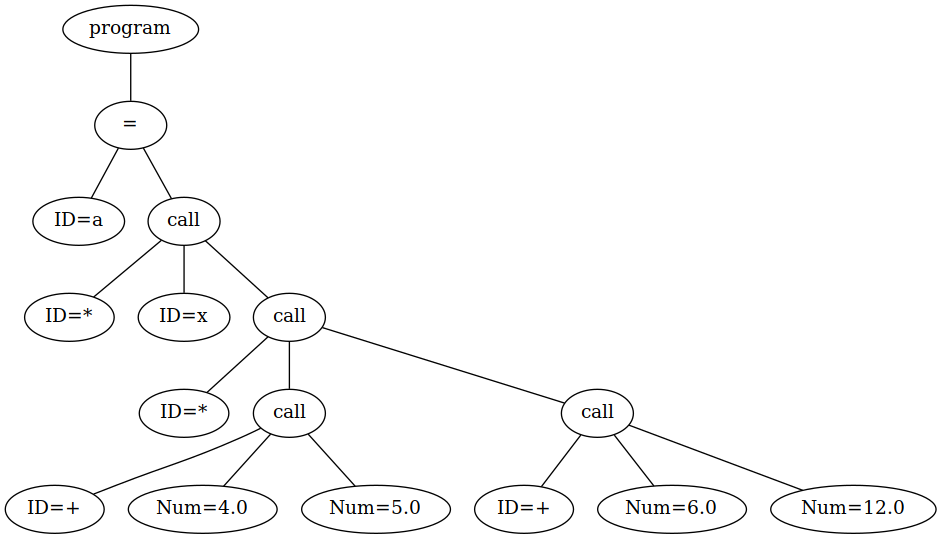
\includegraphics[width=\textwidth*5/6]{3.Theory/images/ast.png}
	\caption{
		Example Abstract Syntax Tree.
	}
	\label{fig:ast}
\end{figure}

The AST from figure \ref{fig:ast} was generated from the following HCL sourcecode:
\begin{lstlisting}[language=HCL,label=lis:typedcls,firstnumber=1]
a = x * (4 + 5) * (6 + 12)
\end{lstlisting}


\subsection{Contextual analysis}
Apart from syntactical analysis, the parser is also concerned with contextual analysis. 
The contextual analysis ensures that types are correct, immutable variables are not reassigned, and other contextual aspects that cannot be inferred from the CFG.
The major part of the contextual analysis is the type checking.

\textbf{Type checking}\\
The type checking part of the parser often utilizes a symbol table, as explained later, in section \ref{sec:symbolTable}.

It is also the responsibility of this portion of the parser to provide any relevant type information that may be needed in order to proceed with compilation in later phases. 
There are several ways to inform the later stages of the compiler about the needed type information. 
One solution is to store and pass the symbol table to the later stages of the compiler. 

Another option is to decorate the AST with the needed type information. 
This is called a decorated syntax tree, and will in most cases be the final output of the parser.
An example of decorating an AST could be when using implicit casts. 
Most languages have this feature between integers and floating point numbers. 
So if the user does arithmetic with an integer and a floating point number, the integer would then be implicitly cast to a floating point number.

\subsection{Single parse and multi parse}
Depending on the language, a single run through the parser may not be enough to validate the input or generate the output. 
For instance, if the language allows for calling of functions or the usage of classes that has not yet been declared.
In this case, the parser should do a single parse to map out the functions and classes that can be used. 
After the first parse another should be done, where the information from the previous parse is utilized to ensure the validity of the input. 

Single pass parsers will usually do more work in the single pass, but overall the single pass parsers will most often be the fastest.
However, a single pass parser do limit the language a bit, and therefore most modern mainstream compilers are multi pass parsers.

\subsection{Parser types}
Generally there are two different approaches to creating a parser.

\textbf{Top down parsing}\\
LL parsers uses a top down parsing strategy. 
LL means that the parser is Left to right using Leftmost derivation. 
If a CFG is LL(K) it means that the parser needs to do, at max, \textit{K} lookaheads in order to parse the sentence. 
LL parsers can be implemented as a table parser, or as a recursive descent parser. 

\textbf{Bottom up parsing}\\
There are a few of different ways to implement bottom-up parsers. 
Namely the LR(K) and the LALR parsers are interesting. 
The bottom-up parsers can recognize a lot more languages than the top-down parsers.
However, they are also generally more complex to implement.
Because of this, bottom-up parsers are only rarely handmade.
They will usually be implemented using the shift-reduce strategy.

\subsection{Parser tools}
Just as with lexers, a vast amount of tools exist in order to ease the parsing part of the compiler. 
The complexity of the parser depends a lot on the type of the language. 
As mentioned, a LL(1) recursive decent parser is fairly simple to develop, whereas a LALR parser is quite tedious to develop. 
Since only a few languages are simple enough to have a handwritten parser pay off, most compilers will often use tool-generated parsers.

However, the group has decided to hand-write the entire compiler, therefore parser generators will not be utilized.
